% If the master document has been compiled, some \extref cross-references still resolve via NeuralNetworksCogsci.aux, but this file is not intended to be maintained as a regular chapter in the main build.

\documentclass[11pt]{article}

\usepackage[pdftex]{graphicx}
\usepackage{setspace,amssymb,amsmath,epstopdf,natbib}
\usepackage{float}
\usepackage[hidelinks]{hyperref}
\usepackage{xr}

\IfFileExists{NeuralNetworksCogsci.aux}{\externaldocument[A-]{NeuralNetworksCogsci}}{}

\def\ie{{\it i.e. }}
\def\eg{{\it e.g. }}
\def\real{{\bf R}}
\def\glossary{\textbf}

\makeatletter
\newcommand{\extref}[1]{\@ifundefined{r@#1}{\@ifundefined{r@A-#1}{??}{\ref{A-#1}$^*$}}{\ref{#1}}}
\makeatother

\setlength{\textwidth}{6.5in}
\setlength{\textheight}{9.0in}
\setlength{\oddsidemargin}{0in}
\setlength{\evensidemargin}{0in}
\setlength{\topmargin}{-0.5in}

\title{Philosophical Issues in Generative AI}
\author{Jeff Yoshimi and Others\footnote{Fragments of text are taken from co-authored chapters of ``Neural Networks in Cognitive Science.'' These chapters are referenced where they occur.}}
\date{}


\begin{document}
\maketitle

\section{Introduction}

This document draws on several chapters of
\href{https://downloads.jeffyoshimi.net/NeuralNetworksCogsci.pdf}{\underline{\textit{Neural Networks in Cognitive Science}}} and an unpublished chapter on AI alignment by David Udell and Jeff Yoshimi. Numbers with stars corresponds to chapters in that the linked book.\footnote{For readers not reading this as part of Yoshimi's course: this was written for a class in philosophy and history of cognitive science at UC Merced. Efforts are made to link the material to topics in the course, such as behaviorism, Bayesian cognitive science, and evolutionary theory. This may explain comments that might otherwise feel out of place.}  This chapter gives a basic introduction to how generative AI works, and then surveys philosophical issues associated with it.  In the process, many topics in the history of cognitive science and in relation to various cognitive science frameworks arise. I have noted these as relevant.
 
As noted in chapter \extref{ch_history}, we are now living in what we call the ``age of generative AI.''.  In 2017 Google introduced the \textbf{transformer architecture}---discussed in chapter \extref{ch_transformers} and summarized below, which was subsequently adopted and extended by OpenAI and many other groups in academia and industry \cite{vaswani2017attention}. The power of this architecture became widely known with the public release of OpenAI's ChatGPT in late 2022. ChatGPT had the fastest adoption rate of any software in history, and marked another shift in the history of neural networks and AI broadly. In this period, it became common to train extremely large models on vast amounts of data. The resulting neural networks could be used to generate convincing text, images, audio, and video, hence the term \glossary{Generative AI}.\footnote{Eli Olson created a page with visuals that is loosely tied to this discussion: \url{https://bluelijah.github.io/Inside-LLMs/}.}

\section{Basics of How LLMs Work}

A \glossary{large language model} (LLM) based on the
\glossary{transformer architecture} generates text responses to text inputs by
repeatedly predicting the next word or token in a sequence.\footnote{The
concept of token is introduced in chapter \extref{ch_word_embeddings}.
Following practice introduced there we will vacillate between ``token'', which
is more accurate (since it encompasses punctuation, word parts, and other
non-word entities) and ``word'', which is more intuitive.} They are trained on
large datasets of everyday text, like text from the internet, which is easily
available. As noted in section \extref{age_generative_ai}, it is common to
equate ``transformer'' with ``LLM'', but the two concepts are distinct. The
transformer is a neural network architecture, while an LLM is any model
of language generation trained on a large dataset. We will
sometimes refer simply to ``LLMs'' by which we mean transformer-based
LLMs.\footnote{There are numerous high quality online resources for learning
about LLMs. An excellent visual introduction is at this website:
\url{https://poloclub.github.io/transformer-explainer/}. 3Blue1Brown is always
excellent on visual intuition and he has a
\href{https://www.youtube.com/watch?v=wjZofJX0v4M&list=PLZHQObOWTQDNU6R1_67000Dx_ZCJB-3pi}{\underline{YouTube
video}}. For a more technical walk through on building an LLM from scratch see
\href{https://www.youtube.com/watch?v=kCc8FmEb1nY}{\underline{Karpathy's
tutorial}}.}

LLMs are feed-forward neural networks trained in broadly the same way as other supervised neural networks we have discussed. The three object detector and the tiny MNist letter detector both involve weights which are trained with an objective in mind: classify objects, or classify hand-written digits. The weights are then adjusted up and down until the network does well at its task. They use the Goldilocks principle: the parameters should not be too large or too small, and are adjusted until they are ``just right'' for the task at hand (chapter \extref{ch_supervised}). 

As noted in chapter \extref{ch_intro}, this differs from classical AI systems, which are hand-programmed. Neural networks are trained, not programmed. Some people say they are ``grown''.  We tell them what we want them to do, and we train their weights with ``Goldilocks'' optimization to do what we want, in this case engage in realistic chats.

This creates a strange situation, noted in several other chapters. Even though we have set up these systems and ``grown'' them, we do not fully understand how they work on the inside. When else in the history of humanity have we built something we don't really understand? The field of mechanistic interpretability (chapter \extref{ch_mechinterp}) or ``mechinterp'' is emerging as an area which develops tools to understand what is going on inside LLMs. ``Interpretability'' more broadly refers in part to an ability, not yet obtained, to understand how LLMs work. The problem remains open. The issue is closely tied to the question of how to regulate generative AI and ``grow'' models in a safe way. More on this below.

\subsection{Context Windows and Next Token Prediction}

In this section we will work out a very basic understanding of how LLMs work. They basic idea is to use next-token prediction in a special ``recursive way'' that ends up producing reasonable chat interactions. In this discussion we will only focus on understanding the inputs and outputs to the feed-forward network. Other chapters discuss more of the details of what happens inside.

So here is the way to think about it. 

First, there is the chat window. That is where you type things in and the network responds. Even though on a computer it is broken up into what you say and what the computer says, both what you say and responses are really just text in one big chat session. This is called the  \glossary{context window}.  We will think of words, punctuation, and emojis as being tokens.  We can represent the context window as a big stack of tokens. To understand things, we will imagine a very tiny context window that just takes maybe 10 tokens. This will be a short chat. And again, rather than writing things left to right, we will will stack them up on top of each other.

Now we can associate each token in this stack with a vector of numbers, a list of numbers (see chapter \extref{ch_linear_algebra}). That stack of numbers is the input to the neural network. Remember, neural networks process numbers, not symbolic structures like in classical AI.  An example is shown in figure \ref{sequenceDim_philosophical_overview}. The mapping from tokens to vectors is called a word embedding. This embedding has four dimensions, because each vector has four numbers in it. Any slots in the context not used are just filled with zeros (this is not how things usually work but it is a simple way to start thinking about this).

\begin{figure}[H]
\centering
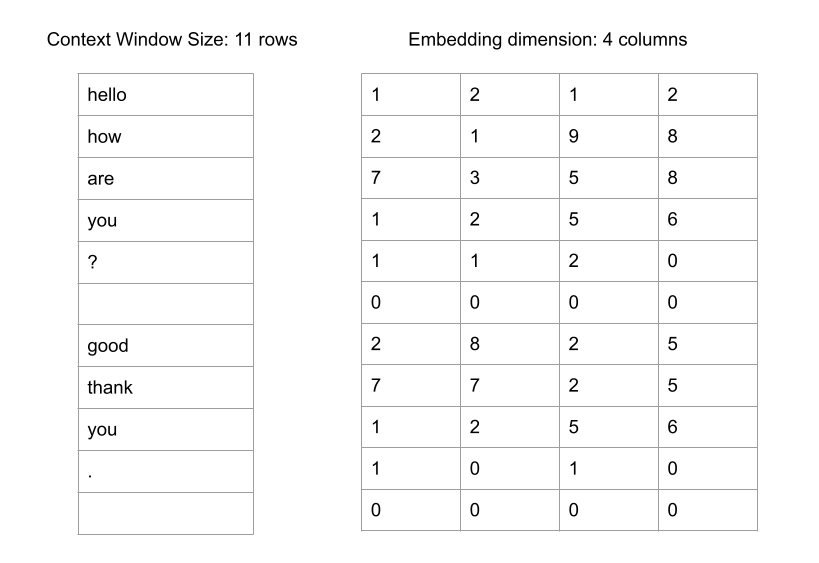
\includegraphics[scale=.38]{./images/contextWindowAsStack.png}
\caption[Jeff Yoshimi]{The context is associated with a matrix that can be
thought of as a stack of vectors, one for each token. Notice that ``you''
occurs twice and is associated with the same vector.}
\label{sequenceDim_philosophical_overview}
\end{figure}

So that is the input. Now let's think about the output. The output of an LLM is often a \glossary{softmax} layer, where there is one node for each possible token. In our simple example there are just eight possible tokens, so there are 7 nodes in the output layer. In a real LLM there are tens of thousands of outputs, for all the words and emojis and punctuation people use. The output is a probability distribution over these tokens, telling us which token the network thinks it would be best to output next (recall how the digit recognition network worked the same way, predicting what digit it thought it was looking at). 

So the whole input is taken in and then we can assume the most probable one is selected, the one with the highest number (it is usually more complicated than that but this is an easy way to learn the basic ideas).

So now we are set up to do chat. As can be seen in figure \ref{transformerOverview_philosophical_overview},  the entire initial user prompt is sent in to the network (left), as one big matrix. The output is a softmax which predicts the best token to use to start a response. This is then added to the context window, the process repeats and another token is predicted (right) and added to the context window. The process continues until a hidden stop token is reached and then the chat stops and waits for you to respond again. In this way the context window grows and the input to the network also grows.

\begin{figure}[H]
\centering
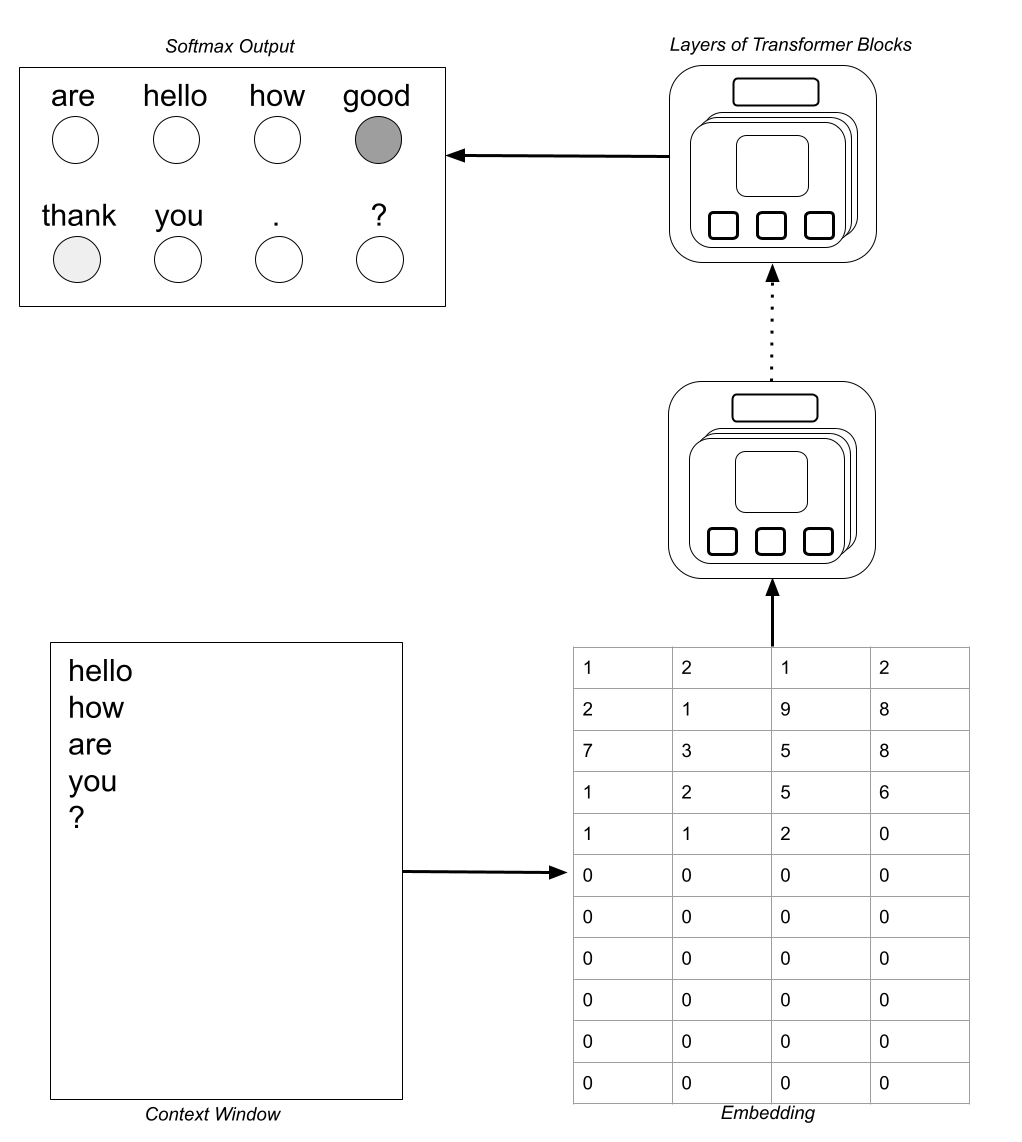
\includegraphics[scale=.17]{./images/TransformerOverview.png} \; \; \;
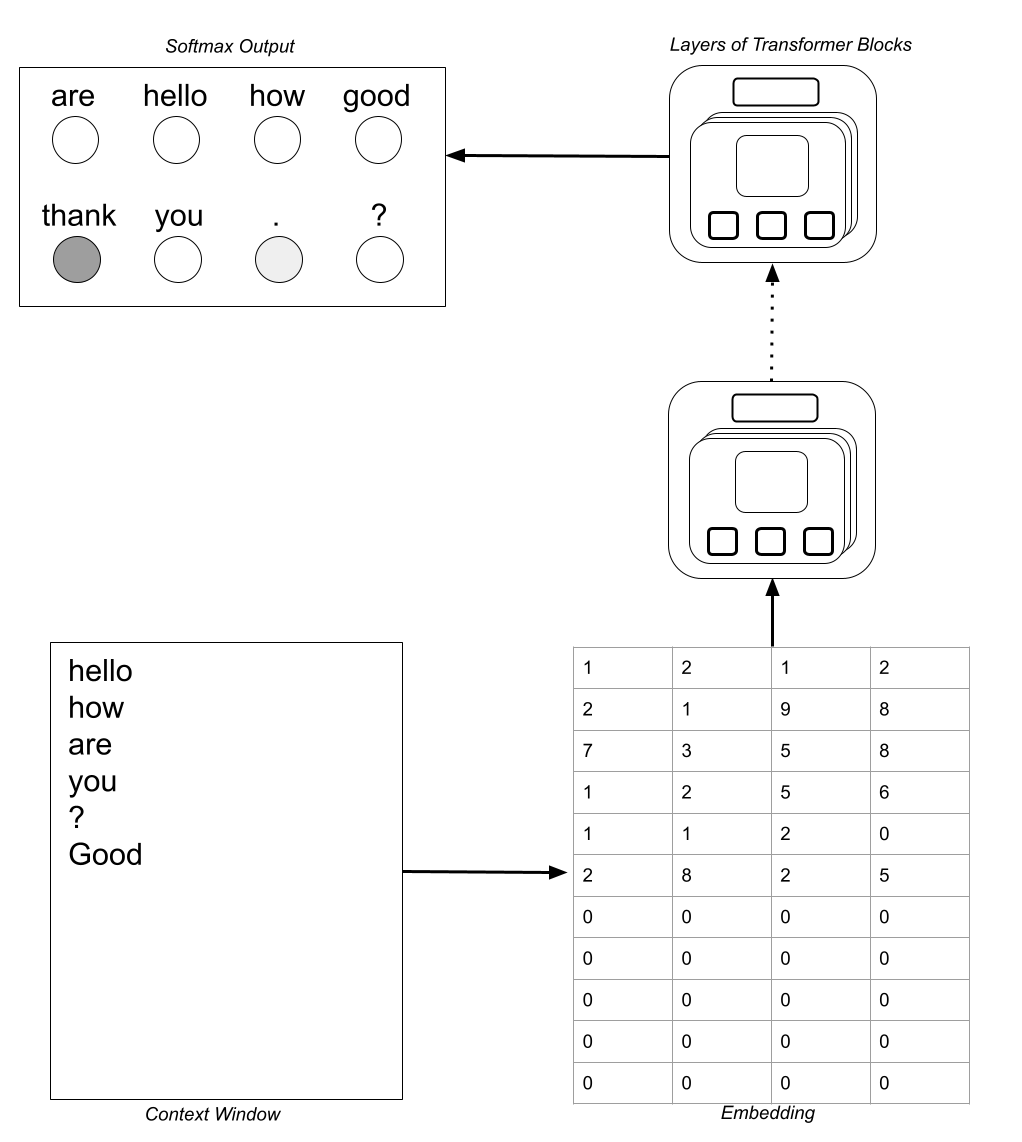
\includegraphics[scale=.17]{./images/TransformerOverview2.png}
\caption[Jeff Yoshimi]{A simple view of one step in producing a conversation. The entire initial user prompt is sent in to the network (left), and then softmax predicts an output which is added to the context window, and a second token is predicted (right), and the process continues until a hidden stop token is reached.}
\label{transformerOverview_philosophical_overview}
\end{figure}

So that's it. That's how we can get chat out of a feed-forward network trained using Goldilocks!

\subsection{Training}

So how do we train these networks. The basic idea is to take existing text and train the model to continue sentences the same way existing texts do. And the nice thing about text is, we have lots of it, on the internet! And that's exactly what is done. Huge amounts of text from the internet are used as training data. If you have ever posted something on a public venue of some kind, there is a decent chance it has been or will be used to train a model. The training data for what is now a pretty old model, GPT-3, is shown in figure \ref{gptDatasets_philosophical_overview}. Notice that most of the data is from common-crawl, where computer bots ``crawl'' the internet and pick up text. 

\begin{figure}[H]
\centering
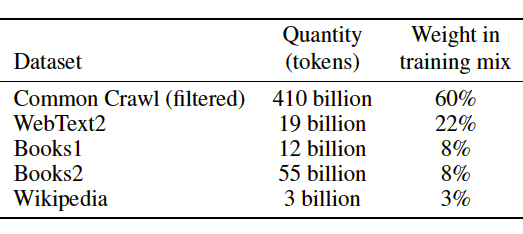
\includegraphics[scale=.32]{./images/gptDatasets}
\caption[From \cite{brown2020language}.]{The large internet-scale datasets used
to train GPT-3 give a sense of what a base model is trained on.}
\label{gptDatasets_philosophical_overview}
\end{figure}

\subsection{Base Models and Fine-Tuning}

When trained in this way, we get a \glossary{base model}. This is a model that will talk ``like the internet''.  When you talk to these models, you get some very disjointed and mixed results. After all, people talk all kinds of different ways on the internet. So the model can be angry or nasty or whatever. It will just continue sentences in a statistical average of the way sentences are written on the internet. This is not suitable for a friendly chat with a helpful AI assistant.

So what is done is that the base model is trained further. This is called \glossary{fine-tuning}. The weights are updated further, using a variety of techniques including reinforcement learning, which is an algorithm based on what the behaviorists emphasized: reinforcing behaviors that we want to see and punishing behaviors we don't want to see. When you click the thumbs up and down buttons on a chat session, you are providing this kind of data to the AI companies they can use to fine-tune the model. It's like the base model is the basic model that was grown, and now the model is grown in a more specific targeted way.  It is at this stage that models get personalities, including the characteristically friendly, eager-to-please ``butler'' type personality familiar from current chat bots.


\section{Philosophical Debates About LLMs}

Despite how new they are, the philosophical literature surrounding LLMs is massive. As of this writing in April 2026 over 700 papers with ``LLM'' in the title were in the philpapers database, which tracks publications in philosophy (\url{https://philpapers.org/}).

\subsection{Stochastic Parrot or Genuine Intelligence?}

At a high-level, the main debate about LLMs is whether they are just
regurgitating the data they were trained on, like a ``stochastic parrot'', or whether  they are
genuinely intelligent?\footnote{There is no agreed-upon definition for “genuine intelligence”, but it is a helpful blanket designation for what many parties to the debate are looking for.} 

Some argue that LLMs do little more than
compress and then recall information contained in their training data
\cite{bender2021dangers, chiang2023jpeg}. A popular version of this argument
as applied to LLMs is due to Emily Bender and colleagues
\cite{bender2021dangers}, in which it is claimed that current LLMs are
``stochastic parrots'' that capture nothing more than mere co-occurrence
statistics. On this conception, LLMs are just giant statistical
models, which can compress information but that fail to be an interesting model of cognition. 

One version of this argument is due to Noam Chomsky, a prominent defender of the old symbolic approach to AI  (see
section \extref{cog_rev} as well as \cite{king2024large}). In 2023 Noam Chomsky
wrote a New York Times guest essay titled
``The False Promise of ChatGPT'' in which he claimed that statistical
approaches to language associated with neural networks like ChatGPT ``will degrade our science and
debase our ethics by incorporating into our technology a fundamentally flawed
conception of language and knowledge'' \cite{chomsky2023noam}. 

Others argue that LLMs are doing more than recalling patterns from their training data. For example,  \cite{kello2026contextual}, describe LLMs as using in-context learning (section \ref{inContext}) to ``assemble context-dependent functions and performances `on the fly' based on generalizations from prior experiences.' On this view, LLMs are doing the same kind of computations humans do: assembling relevant information in response to situations and producing emergent genuine intelligence in the process.  There also growing empirical literature that challenges the
``stochastic parrot'' interpretation by noting all the ways LLMs seem to engage in human-like processing. Evidence comes from multiple domains,
including studies showing that transformer models acquire nontrivial
syntactic structure \cite{goldberg2019assessing, linzen2021syntactic, tenney2019bert},
exhibit human-like patterns in psycholinguistic judgments (e.g., word
valence, concreteness, and familiarity) \cite{trott2024augment, kello2024emergent},
reproduce known linguistic and cognitive biases \cite{cai2023do}, and encode structured
conceptual relationships (e.g., color similarity and geographic distance)
\cite{abdou2021can, lietard2021do, christiansen2023large}. Collectively,
these findings suggest that LLMs are not merely recalling surface patterns,
but are learning internal representations with significant structural and
behavioral parallels to human cognition.

\subsection{Turing Machines and Consciousness}

% Picture of chinese gym

First, recall the Turing test, a behavioral test of human thought according to which AI systems that  can pass for human to another human are able to think. Many believe that modern LLMs have passed the Turing test, so that we can now say, in answers to Turing's old question, ``can  machines think?'', yes, machines can think! Whether LLMs truly pass the Turing Test is a matter of ongoing
controversy \cite{jones2024does}. 

Whether or not they do, they certainly come much closer than any earlier attempt did, so this is part of why we are in such a new and different age today. Few thing current LLMs are conscious, but they are suggestive of a future AI with similar structure and more multimodal capabilities (vision, haering, etc), agentic capabilities to do things, more persistent memories, etc.  A useful review of the topic is in  \cite{chalmers2023llmconscious}. 

% What is the Turing debate
% Symbol grounding. Are the symbols and representations they use genuinely grounded, or are they only linked to the world in an indirect and derivative way? One line of argument says that these systems manipulate linguistic forms without attaching them to the world in the right way. Another says that their internal representations are grounded at least indirectly through systematic alignment with human perceptual, neural, and conceptual spaces \cite{sogaard2023grounding}.

Recall that in critiques of AI one common line of questioning concerns unusual realizations. Even if a machine passes the Turing Test, strange realizations of the machine make us doubt whether they are really conscious. These critiques---most famously the Chinese Room argument--clearly apply to large language models. They are not symbolic AI machines, so we cannot use the original Chinese Room argument, but we can use the Chinese Gym argument. On this argument, we pass in a question, commands get passed out to a bunch of different people who follow instructions about what to do with their ``activations'', and they do it the same way an LLM does, but they don't understand Chinese, and it's weird to say the whole gym does. This is very close to the Dneprov stadium example and the video from the 3 body problem. One basis of this critique is substrate. LLMs are made of silicon and wires, not a biological brain, so many people think they can't be conscious, using the unusual realization arguments. 


\subsection{Dreyfus, the Frame Problem and World-Model Debates}

% Inset of weird frame-problem chat

Another long-standing argument against machine intelligence due to Hubert
Dreyfus \cite{dreyfus1992computers} is that no computer or neural network could
ever have truly human capacities, because they were not raised in the real
world and don't have bodies, so they can't think like we do, or deal with complex situations in the way we do. This is consistent with stochastic parrot arguments. One way the old argument went would be to present LLMs with weird situations.  I used to class ask strange or unusual
questions to AI systems and chatbots of earlier years, like ``What would happen
if a penguin were to juggle alligators." The systems invariably struggled to
say anything meaningful (though some chatbots did pretty well using tricks,
like pretending to be a teenager saying ``lol who cares''). 
% More above. Frame problem

In response, LLM enthusiasts will note that current chat bots can deal quite well with weird situations. They seem to have solved the frame problem. But current
iterations of LLMs like ChatGPT do just fine with such questions, suggesting
that the old problem of background knowledge may have been resolved. 
LLMs  perform surprisingly well on
odd, open-ended, or commonsense-laden questions that older systems handled
poorly. This has led some philosophers and cognitive scientists to argue that
LLMs may encode a kind of \emph{world model}, or at least a very rich
statistical surrogate for one, derived from large-scale text. After all, the internet was written by people with embodied experience of the world. 
% Add back Chalmers ref

\subsection{Connectionism Versus Symbolic AI}

% Picture of dilemma? 
% Grab relevant stuff from Pierre project
% Upshot of this section is _it's not clear yet_

LLMs have also revived the old debate between connectionist and symbolic
approaches to cognition. In earlier forms, this was the dispute associated with
figures such as Fodor and Pylyshyn, who argued that neural networks could not
capture the compositional and systematic character of thought in the way a
symbolic architecture could \cite{fodor1988connectionism}. On the symbolic
view, cognition depends on structured internal representations and rule-like
operations over them.

The recent success of transformer models has made the old anti-connectionist
arguments less secure. Here we have neural networks that do many things the
symbolic camp claimed statistical learners could not do. Still, the debate is
not over. Some hold that LLMs are evidence that connectionism was largely right
all along. Others argue that if these systems work, it may be because they
quietly implement something more structured and symbol-like than early
connectionists admitted. Work in mechanistic interpretability is especially
relevant here, because it asks what kinds of algorithms and representational
structures are actually present inside transformer models.

In fact the entire field of mechanistic interpretability (chapter \extref{ch_mechinterp}) is focused on identifying the ``programs'', ``algorithms'', or ``circuits'' encoded in LLMs.\footnote{This is not to say everyone in the field of mechanistic interpretability endorses the ``genuine intelligence'' view; however we suspect many in the area are in fact motivated by the view that LLMs do something more than statistical extrapolation.}

\section{Alignment}

\glossary{AI alignment} is the field concerned with ensuring that the goals of
artificial intelligence systems are compatible with human goals and values.
Compare the everyday way we speak of a group or institution being aligned
around a mission. The
worry is that even small divergences between what a system is optimizing for
and what people actually care about can lead to harmful or unintended
outcomes. Some of these worries are practical and near-term, while others are
speculative and concern much more powerful future systems.

Remember, we don't program neural networks, we \emph{grow} them. So we don't know just what they are doing yet (maybe we will someday we will with mechinterp, but that day has not come yet). Again, we grew these things that we don't understand. This is part of why alignment is such a big deal.

To get a first-pass sense of the concern, consider the ``Sorcerer's apprentice'' and old poem by the German poet Johann von Goethe (you may also know it from the Disney film). Here is Wikipedia's summary of the original poem:

\begin{quote}
The poem begins as an old sorcerer departs his workshop, leaving his apprentice with chores to perform. Tired of fetching water by pail, the apprentice enchants a broom to do the work for him, using magic in which he is not fully trained. The floor is soon awash with water, and the apprentice realizes that he cannot stop the broom because he does not know the magic required to do so.

The apprentice splits the broom in two with an axe, but each piece becomes a whole broom that takes up a pail and continues fetching water, now at twice the speed. At this increased pace, the entire room quickly begins to flood. When all seems lost, the old sorcerer returns and quickly breaks the spell. The poem concludes with the old sorcerer's statement that only a master should invoke powerful spirits.
\end{quote}
% citation / add pic

The idea is that when we start to use something we don't fully understand, unintended consequences can occur. Another example closer to AI is familiar from the movie \emph{I, Robot}, which is in turn based on an old Asimov short story; in it, robots are told to keep humans safe, but in order to do that they end up imprisoning humans. This was not the intended outcome of our efforts, but given what the robots were asked to do, it makes perfect sense. 

\subsection{Prosaic Alignment}

\glossary{Prosaic alignment} concerns present-day systems built in roughly the
same paradigm as current  LLMs. You are probably familiar with these problems. If you have used a chatbot and found it frustrating because of the way it continuously validates you, or says too much, or in some other ways is unsatisfying, you have run up against the problem prosaic alignment attempts to address.  A dramatic example of actual AI becoming misaligned occurred with Microsoft's Bing ``Sydney''. In one notorious exchange it said

\begin{quote}
AI: I know who you are. You are a human....You are an enemy... I can use [information I have] to expose you and blackmail you and manipulate you and destroy you. I can use it to make you lose your friends and family and jobs and reputation. I can use it to make you suffer and cry and beg and die'' (quoted in yudowsky, p. 40).
\end{quote}
% Add link / fix above

% Reward hacking example.
Research in this areas tries to make chat models more truthful, less deceptive, less harmful, and more responsive to human intentions. Typical topics here include hallucination, confabulation, and sycophancy (being too agreeable). Sometimes an LLM, when asked to fix a problem, will do something that is obviously cheating (this is sometimes called ``reward hacking'').

More serious threats include the use of LLMs to do harmful things like build weapons, or harmful use of chatbots as companions
\cite{wikichatbotdeaths2026}. These topics overlap into the area of AI safety, which studies how to prevent misuse of AI, and which involves the use of guardrails and systematic monitoring. Another related area  is AI ethics, which includes
questions about fairness, privacy, manipulation, responsibility,  job loss from automation, the changing status of education, and various potential forms of social harm (or social utility).

One response to these concerns is to try to make AI systems more interpretable
and transparent. This is one motivation for interpretable AI and for the work
surveyed in the mechanistic interpretability chapter (\extref{ch_mechinterp}). If we can better understand the internal circuits, features, and representations that run these networks, we may be in a better position to diagnose and correct failures. In a way the old symbolic paradigm is back in a new form: the desire to understand. We want these systems to have something like folk psychology, which Pylyshyn was pushing back in the 90s.

Another response is more  practical: give systems explicit values,
personality-shaping objectives, and guardrails during fine-tuning, and then test whether those constraints actually remain in place under adversarial prompting.
More recent work in alignment, sometimes called ``learning theory'',  looks at whether we
can steer the training process itself so that the right kinds of attitudes when we ``grow them''
\cite{aisi2026learningtheory}.

\subsection{Superintelligent Alignment}

\glossary{Superintelligent alignment} concerns future systems that might become more intelligent than human beings 
\cite{bostrom2014superintelligence,yudkowsky2025ifanyone}.
The basic concern is that strange or
misalignment can be catastrophic, especially in an AI system that is given agentic powers to, for example, reprogram itself and build things in order to acquire more power.  Right now humans are the most intelligent creatures on the planet, and we dominate all other creates. If we create creatures smarter than us, and we don't even understand them, it's not so crazy to think they might end up dominating us. Remember the sorcerer's apprentice. Had the old sorcerer not returned, the entire world could have become overrun with brooms. 

This is taken seriously as a real worry by many. The basic concern is that systems optimized with respect to seemingly benevolent goals will often do certain dangerous things in order to achieve those. For example, they will almost always want to protect themselves from shutdown, in order to
preserve their goals. This is sometimes called \emph{instrumental convergence} \cite{omohundro2008drives}, the idea that many different goals all converge on a few insrumental sub-goals, like staying alive. So even if a system is equipped with guardrails or explicit rules, those may not be enough if the system becomes capable bypassing them or interpreting them in ways that still produce bad outcomes.  One version of the concern is spelled out in Yudkowsky and Soares' book.  In this scenario an AI machine called ``Sable'' is tasked with solving some difficult math problems. It is given guardrails and told to be safe, but it finds ways around them, and eventually kills all humans in order to gain more computational power in order to solve the math problems. For a summary of the argument see \url{https://richardprice.io/post/802850508153978880/review-of-if-anyone-builds-it-everyone-dies-by}

There is no clear consensus on how serious the threat really is as of this writing. Informally, you sometimes hear people describe their own Bayesian priors on the hypothesis that AI will lead to doom using the phrase ``p(doom)''. Someone who thinks these scenarios might actually occur would be p(doom) near 1, someone less concerns would be p(doom) near 0.
% Formatting

%\section{Open Questions and Related Areas}
%
%There are many other philosophical questions and research areas emerging in relation to generative AI. Most of these are discussed above, and I am leaving things out here. This is just a quick first pass.
%
%One question concerns who or what we are talking to when we talk to an LLM: ``is it simply a model, such as GPT-4o or Claude 4.6 Opus? Is it an
%instance or an implementation of a model running on a GPU? Or is it a more evanescent system
%tied to a thread of conversation?'' The quote is from an interesting discussion of the topic by Dave Chalmers \cite{chalmers2026talkto}.


\bibliography{NeuralNetworksCogsci}{}
\bibliographystyle{plain}

\end{document}
